\documentclass[12pt]{article}
\usepackage[utf8]{inputenc}
\usepackage{amsmath}
\usepackage{amsfonts}
\usepackage{amssymb, bm}
\usepackage{tikz}
\usetikzlibrary{calc,arrows,positioning,shapes,shapes.gates.logic.US,trees, backgrounds}

% ==========
% = Floats =
% ==========
\usepackage{float}
% include external pictures
\usepackage{graphicx} %Graphics/figures
% rotate figures/tables
\usepackage{rotating} 
% For professional tables
\usepackage{booktabs,threeparttable, multirow} 
\usepackage{tabularx}
% For fixing the column widths
\usepackage{array}
\newcolumntype{L}[1]{>{\raggedright\let\newline\\\arraybackslash\hspace{0pt}}m{#1}}
\newcolumntype{C}[1]{>{\centering\let\newline\\\arraybackslash\hspace{0pt}}m{#1}}
\newcolumntype{R}[1]{>{\raggedleft\let\newline\\\arraybackslash\hspace{0pt}}m{#1}}

\usepackage[margin=1in]{geometry}
% \setlength{\parindent}{0.5in}

\begin{document}

A relatively complete description of the random effects (latent variables) for each level of a relatively simple MLTA with two timepoints and three classes is shown in Figure \ref{fig:3c-re}.
\begin{figure}[ht]
\centering
\scriptsize
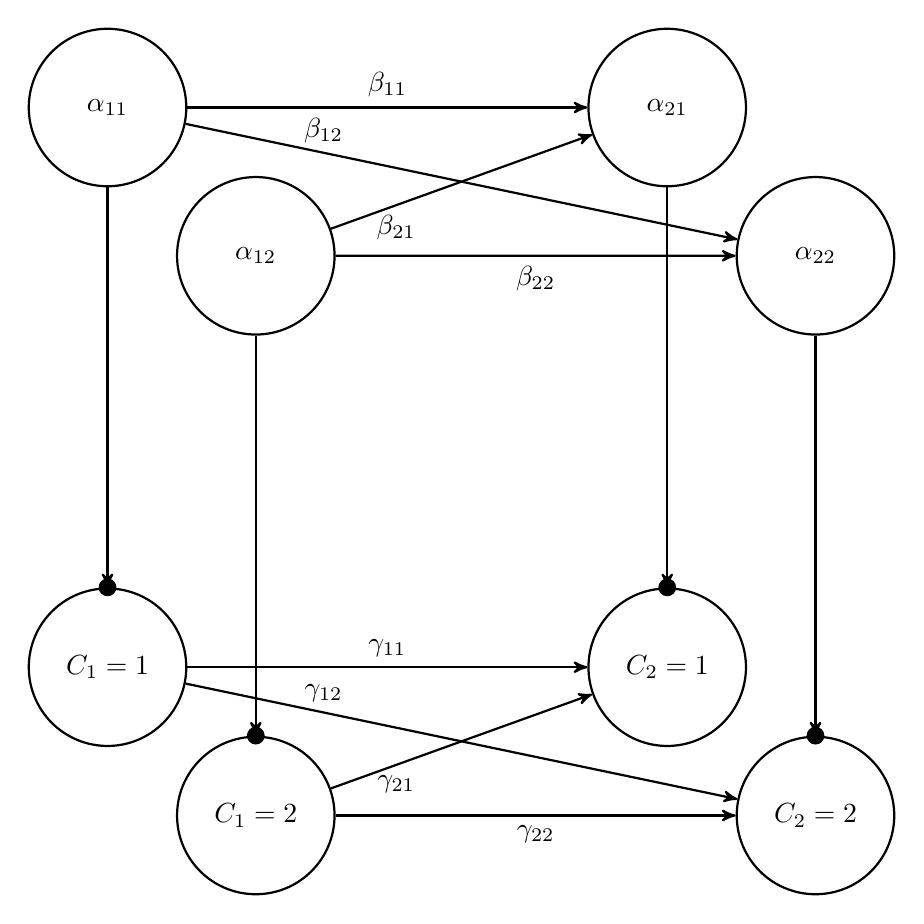
\begin{tikzpicture}[auto,scale=2,
	latent/.style={circle,draw,thick,inner sep=0pt,minimum size=20mm},
	error/.style={circle,inner sep=0pt,minimum size=10mm},
	manifest/.style={rectangle,draw,thick,inner sep=0pt,minimum size=10mm},
	corr/.style={<->,>=stealth', bend right=30},
	intercept/.style={regular polygon,
        regular polygon sides=3,draw,thick,inner sep=0pt,minimum size=10mm},
	mean/.style={regular polygon,regular polygon sides=3,draw,thick,inner sep=0pt,minimum size=20mm},
	paths/.style={->, thick, >=stealth'},
	variance/.style={<->, thick, >=stealth', bend left=270},
	varianceTop/.style={<->, thick, >=stealth', bend right=270, looseness=2},
	unique/.style={<->, thick, >=stealth', loop above=270, looseness=8},
	factvar/.style={<->, thick, >=stealth', loop below=90, looseness=8},
	ghost/.style={rectangle,draw,thick,inner sep=0pt,minimum size=0mm},
	dots/.style={rectangle,draw,thick,inner sep=0pt,minimum size=2mm, color=white, text=black}
	]
\tikzset{mystyle/.style={->,double=black}} 
% latent classes
\node [latent] (c11) {$C_1=1$};
\node [latent] (c12) [below right = .25in of c11] {$C_1=2$};
\node [latent] (c21) [right = 2in of c11] {$C_2=1$};
\node [latent] (c22) [right = 2in of c12] {$C_2=2$};

\node [latent] (a11) [above = 2in of c11] {$\alpha_{11}$};
\node [latent] (a12) [above = 2in of c12] {$\alpha_{12}$};
\node [latent] (a21) [above = 2in of c21] {$\alpha_{21}$};
\node [latent] (a22) [above = 2in of c22] {$\alpha_{22}$};

% random intercepts 
\filldraw (c11.north) circle[radius=1.5pt];
\filldraw (c12.north) circle[radius=1.5pt];
\filldraw (c21.north) circle[radius=1.5pt];
\filldraw (c22.north) circle[radius=1.5pt];

% gamma paths
\draw [paths] (c11) to node {$\gamma_{11}$} (c21);
\draw [paths] (c11) to node[near start, above] {$\gamma_{12}$} (c22);
\draw [paths] (c12) to node[near start, below] {$\gamma_{21}$} (c21);
\draw [paths] (c12) to node[below] {$\gamma_{22}$} (c22);

% level-2 regression weights (betas)
\draw [paths] (a11) to node {$\beta_{11}$} (a21);
\draw [paths] (a11) to node[near start, above] {$\beta_{12}$} (a22);
\draw [paths] (a12) to node[near start, below] {$\beta_{21}$} (a21);
\draw [paths] (a12) to node[below] {$\beta_{22}$} (a22);

% draw lines connecting levels
\draw [paths] (a11) to node {} (c11);
\draw [paths] (a12) to node {} (c12);
\draw [paths] (a21) to node {} (c21);
\draw [paths] (a22) to node {} (c22);


%\draw [unique] (a11) to node {$\textrm{var}\left(\alpha_1\right)$} (a1);
%\draw [unique] (a22) to node {$\textrm{var}\left(\alpha_2\right)$} (a2);
\end{tikzpicture}
\caption{Conceptual diagram of latent variables in a 3-class MLTA.}\label{fig:3c-re}
\end{figure}

Next, we have demonstrated how the variance is decomposed for the calculation of a variety of $R^2$ like measures associated with the latent class at time 2.

\section{Variance decomposition}

Some general notation.

\begin{itemize}
\item K = number of latent classes, $1, 2,..., k, ..., K$, where latent class $K$ is the reference class.
\item $K-1$ random intercepts needed to separate the classes
\item $\alpha_{tk}$ random intercept for timepoint $t$ of class $k$, so $\alpha_{11}$ is the random intercept of class $1$ at timepoint $1$.
\item $C_t$ is latent class at time $t$, which takes on values $C_t = 1, 2, ..., k, ..., K$
\item $\beta_{k_{t} j_{t+1}}$ represents the regression weight associated with latent class $k$ at timepoint $t$ as a dummy-coded predictor of latent class $j$ at timepoint $t+1$; ex. $\beta_{11}$ is the regression weight of latent class 1 at timepoint 1 predicting latent class 1 at timepoint 2. The same scheme applies to $\gamma$ parameters.
\item $\frac{\pi^2}{3} = 3.29$ is the variance of the logistic distribution
\end{itemize}

Next, the decomposition is broken down. To help with showing how this works, we used the simulation condition detailed in Table \ref{tb:mlta-model}.

\begin{table}[!htp]
\centering
\begin{threeparttable}
\caption{Model details for example calculations}
\label{tb:mlta-model}
\begin{tabular}{l r c r r r r}
\toprule
& & & \multicolumn{3}{c}{Transition Matrix}\\ \cmidrule(lr){4-7}
\multicolumn{2}{l}{Class Size} & & $C_{(t-1)\setminus t}$ & $C_2 =1$ & $C_2 =2$ & $C_2 =3$   \\ \midrule
\multicolumn{7}{c}{Probability Scale}\\
$C_1 =1$	& 0.30 & &  $C_1 =1$	& 0.60  & 0.37 & 0.03 \\
$C_1 =2$	& 0.50 & &  $C_1 =2$	&  0\tnote{b}     & 0.78 & 0.22\\
$C_1 =3$	& 0.20 & &  $C_1 =3$	&  0\tnote{b}     & 0\tnote{b}     & 1\\
\multicolumn{7}{c}{Logit Parameterization}\\
$C_1 =1$	& $0.40$   & & $C_1 =1$	&  $3.12$ &  $2.62$ & 0\tnote{a}\\
$C_1 =2$	& $0.90$    & & $C_1 =2$	& $-15$\tnote{b} &  $1.27$ & 0\tnote{a} \\
$C_1 =3$	& 0\tnote{a} & & $C_1 =3$	& $-15$\tnote{b} &  $-15$\tnote{b} & 0\tnote{a} \\ \midrule
\multicolumn{3}{l}{Random Effects\tnote{c}} & &\multicolumn{3}{r}{Regression Weights}\\ 
\multicolumn{3}{l}{$\mathrm{var}(\alpha_1) = 0.8$} & &\multicolumn{3}{r}{${\bm \gamma} = (18, 17.5,$ 0\tnote{b} $, 16)$}\\ 
\multicolumn{3}{l}{$\mathrm{var}(\alpha_2) = 0.25$} & &\multicolumn{3}{r}{${\bm \beta} = (0.3, 0.3,$ 0\tnote{b} $, 0.3)$}\\
 \bottomrule
\end{tabular}
% \vspace*{1mm}
 	\begin{tablenotes}[para, flushleft]
    {\small
        \textit{Note.} \ \item[a]parameter fixed for identification; \item[b]parameter fixed for stage sequential development hypothesis; and \item[c]random effects were assumed invariant across latent class intercepts.
    }
 	\end{tablenotes}
 \end{threeparttable}
\end{table}


\begin{enumerate}
\item ICC for latent class at time 1. Which is actually 2 ICC values

\begin{align*}
ICC_1 &= \frac{\mathbb{V}(\alpha_{11})}{\mathbb{V}(\alpha_{11}) + \frac{\pi^2}{3}}=\frac{0.8}{0.8 + 3.29}=0.20\\
ICC_2 &= \frac{\mathbb{V}(\alpha_{12})}{\mathbb{V}(\alpha_{12}) + \frac{\pi^2}{3}}=\frac{0.8}{0.8 + 3.29}=0.20
\end{align*}

\item Compute the variance of latent class at time 1 or $\mathbb{V}(C_1)$. We did this using the following:

First, using the expected value of the intercepts $\alpha_{11}=0.40$, $\alpha_{12}=0.90$, and $\alpha_{13}=0$ we transformed these into probabilities.
\begin{align*}
\pi_{1}=Pr(C_1 =1) &= \frac{\exp(\alpha_{11})}{\sum_{k=1}^K\exp(\alpha_{1k})}\\
 &= \frac{\exp(\alpha_{11})}{\exp(\alpha_{11}) + \exp(\alpha_{12}) + 1}=0.301\\
\pi_{2}= Pr(C_1 =2) &=  \frac{\exp(\alpha_{12})}{\exp(\alpha_{11}) + \exp(\alpha_{12}) + 1}=0.497\\
\pi_{3}= Pr(C_1 = 3) &= 1 - Pr(C_1=1) - Pr(C_1=2)=0.202
\end{align*}
Next, we use these to compute the variance using the definition of variance:
\begin{align*}
\mathbb{V}(C_1) &= \mathbb{E}(C_1^2) - [\mathbb{E}(C_1)]^2\\
 &= \left[1^2\times Pr(C_1 =1) + 2^2\times Pr(C_1 =2) + 3^2\times Pr(C_1 =3) \right] -\\&\qquad \left[1\times Pr(C_1 =1) + 2\times Pr(C_1 =2) + 3\times Pr(C_1 =3)\right]^2\\
 &= \left[0.301 + 1.987 + 1.818\right] - \left[0.301 + 0.993 + 0.606\right]^2\\
 &= 0.493
\end{align*}

\item Compute the contribution of $C_1$ variance on $C_2$ variance. Meaning, how much of the variance of latent class at time 1 gets forwarded to latent class at time 2. This is here Figure \ref{fig:3c-re} becomes really handy.
The most difficult part of this is adequately accounting for the correlation among transition paths at level-1.

Here, the variance of $C_1$ is transferred forward in two components: towards $C_2=1$ and $C_2=2$ and this can occur by a path from $C_1=1$ and $C_1=2$. 
All four regression weights ($\gamma$'s) get utilized here.
I denoted this $\mathbb{V}(C_{1\rightarrow 2})$, the variance of $C_1$ forwarded to $C_2$.
\begin{align*}
\mathbb{V}(C_{1\rightarrow 2})&= \mathbb{V}(C_{1\rightarrow 21}) + \mathbb{V}(C_{1\rightarrow 22})
\end{align*}
meaning that forwarded variance is the sum of the forwarded variances to each latent class.

\begin{align*}
\mathbb{V}(C_{1 \rightarrow 21}) &= (\alpha_{21} +\gamma_{11})^2\mathbb{V}(C_{11}) + \gamma_{21}^2\mathbb{V}(C_{12}) + \gamma_{11}\gamma_{21}\mathbb{COV}(C_{11}, C_{12})\\
&= \gamma_{11}^2\pi_{1}(1-\pi_{1}) + \gamma_{21}^2\pi_{2}(1-\pi_{2}) - \gamma_{11}\gamma_{21}\pi_{1}\pi_{2}\\
&=68.2\\
\mathbb{V}(C_{1 \rightarrow 22}) &= \gamma_{12}^2\mathbb{V}(C_{11}) + \gamma_{22}^2\mathbb{V}(C_{12}) + \gamma_{12}\gamma_{22}\mathbb{COV}(C_{11}, C_{12})\\
&= \gamma_{12}^2\pi_{1}(1-\pi_{1}) + \gamma_{22}^2\pi_{2}(1-\pi_{2}) - \gamma_{12}\gamma_{22}\pi_{1}\pi_{2}\\
&= 86.6	\\
\mathbb{V}(C_{1\rightarrow 2})&= \mathbb{V}(C_{1\rightarrow 21}) + \mathbb{V}(C_{1\rightarrow 22})\\
&=\gamma_{11}^2\pi_{1}(1-\pi_{1}) + \gamma_{21}^2\pi_{2}(1-\pi_{2}) - \gamma_{11}\gamma_{21}\pi_{1}\pi_{2} +\\
&\qquad \gamma_{12}^2\pi_{1}(1-\pi_{1}) + \gamma_{22}^2\pi_{2}(1-\pi_{2}) -  \gamma_{12}\gamma_{22}\pi_{1}\pi_{2}\\
&= \left(\gamma_{11}^2+\gamma_{12}^2\right)\pi_{1}(1-\pi_{1}) + \left(\gamma_{21}^2+ \gamma_{22}^2\right)\pi_{2}(1-\pi_{2}) -\\
&\qquad \left(\gamma_{11}\gamma_{21}+\gamma_{12}\gamma_{22}\right)\pi_{1}\pi_{2}\\
&= 132.7 + 64.0 - 41.9\\
&= 154.8
\end{align*}

\item Split forwarded variance of $C_1$ by the $ICC_k$ associated with each random intercept at time 1.
This breaks the variance passed forward into two pieces. The first, $\mathbb{V}(C_{1\rightarrow 2}^{+})$, represents the amount of variance explained by the level-2 intercept variances.
The second, $\mathbb{V}(C_{1\rightarrow 2}^{-})$,  represents the amount of residual (unexplained) forwarded variance by the inclusion of the random effects.

\begin{align*}
\mathbb{V}(C_{1\rightarrow 2}^{+}) &= ICC_1\times\left[\left(\gamma_{11}^2+\gamma_{12}^2\right)\pi_{1}(1-\pi_{1}) - \left(\gamma_{11}\gamma_{21}\right)\pi_{1}\pi_{2}\right] + \\
&\qquad ICC_2\times\left[\left(\gamma_{21}^2+ \gamma_{22}^2\right)\pi_{2}(1-\pi_{2}) - \left(\gamma_{12}\gamma_{22}\right)\pi_{1}\pi_{2}\right]\\
&= 0.20(132.7-0) + 0.20(64.0-41.9)= 30.3\\
\mathbb{V}(C_{1\rightarrow 2}^{-}) &= (1-ICC_1)\times\left[\left(\gamma_{11}^2+\gamma_{12}^2\right)\pi_{1}(1-\pi_{1}) - \left(\gamma_{11}\gamma_{21}\right)\pi_{1}\pi_{2}\right]\\
&\qquad (1-ICC_2)\times\left[\left(\gamma_{21}^2+ \gamma_{22}^2\right)\pi_{2}(1-\pi_{2}) - \left(\gamma_{12}\gamma_{22}\right)\pi_{1}\pi_{2}\right]\\
&= 0.80(132.7-0) + 0.80(64.0-41.9) = 124.5
\end{align*}

\item Next, we need to break down the contribution of $\alpha_1$ on $C_2$. $\alpha_1$ influence $C_2$ indirectly through $C_1$ and $\alpha_2$.

\begin{itemize}
\item[i.] Contribution of $\alpha_1$ on $C_2$ through $C_1$

This is the piece computed in part 4: $\mathbb{V}(C_{1\rightarrow 2}^{+})$
\item[ii.] Contribution of $\alpha_1$ on $C_2$ through $\alpha_2$

Here, we utilize a system similar to part 3 in order to account for the variance in both intercepts. However, because these are all on the logit scale and are random effects, we have no covariance in this case. In theory, one could be specified, though.

\begin{align*}
\mathbb{V}(\alpha_{1\rightarrow 2})&= \mathbb{V}(\alpha_{1\rightarrow 21}) + \mathbb{V}(\alpha_{1\rightarrow 22})
\end{align*}
where we similarly pass the variance in $\alpha_1$ to $\alpha_2$ in two pieces.

\begin{align*}
\mathbb{V}(\alpha_{1 \rightarrow 21}) &= \beta_{11}^2\mathbb{V}(\alpha_{11}) + \beta_{21}^2\mathbb{V}(\alpha_{12})\\
&= 0.3^2(0.8) + 0^2(0.8)\\
&= 0.07\\
\mathbb{V}(\alpha_{1 \rightarrow 22}) &= \beta_{12}^2\mathbb{V}(\alpha_{11}) + \beta_{22}^2\mathbb{V}(\alpha_{12})\\
&= 0.3^2(0.8) + 0.3^2(0.8)\\
&= 0.14\\
\mathbb{V}(\alpha_{1\rightarrow 2})&= \mathbb{V}(\alpha_{1\rightarrow 21}) + \mathbb{V}(\alpha_{1\rightarrow 22})\\
&=  0.21
\end{align*}
\end{itemize}
Lastly, we just need to get the total contribution of $\alpha_1$ on $C_2$ by adding these pieces together.
\begin{align*}
\mathbb{V}(\alpha_1\rightarrow C_2) &= \mathbb{V}(C_{1\rightarrow 2}^{+}) + \mathbb{V}(\alpha_{1\rightarrow 2}) + \mathbb{COV}(C_{1\rightarrow 2}^{+}, \alpha_{1\rightarrow 2})\\
&=  \mathbb{V}(C_{1\rightarrow 2}^{+}) + \mathbb{V}(\alpha_{1\rightarrow 2}) + 2\sqrt{\mathbb{V}(C_{1\rightarrow 2}^{+})\times \mathbb{V}(\alpha_{1\rightarrow 2})}\\
&= 30.3 + 0.2 + 5.0\\
&= 35.5
\end{align*}

\item Variance of $C_2$ with respect to class size.

Next, we need to get the variability in $C_2$ that is based on the class sizes at timepoint 2. This is tedious but not hard.
First, we used the intercepts at both timepoints to compute the transition logits. That is we first get the transition probabilities then use those to get the class proportions.
The transition matrix is found by $\mathrm{logit}[\tau_{k_t j_{t+1}}]$ as the transition logit from class $k$ at time $t$ to class $j$ at time $t+1$.
\begin{align*}
\mathrm{logit}[\tau_{11}] &= \alpha_{21} + \beta_{11}\alpha_{11} + \gamma_{11} = 3.12\\
\mathrm{logit}[\tau_{12}] &= \alpha_{21} + \beta_{12}\alpha_{11} + \gamma_{12} = 2.62\\
\mathrm{logit}[\tau_{13}] &= 0\\
\mathrm{logit}[\tau_{21}] &= \alpha_{22} + \beta_{21}\alpha_{12} + \gamma_{21}=-15\\
\mathrm{logit}[\tau_{22}] &= \alpha_{22} + \beta_{22}\alpha_{12} + \gamma_{22}=1.27\\
\mathrm{logit}[\tau_{23}] &= 0\\
\mathrm{logit}[\tau_{31}] &= \alpha_{21}=-15\\
\mathrm{logit}[\tau_{32}] &= \alpha_{22}=-15\\
\mathrm{logit}[\tau_{33}] &= 0
\end{align*}
which in turn results in the transition probabilities given in Table \ref{tb:mlta-model}, repeated here as

\begin{table}[!htp]
\centering
\begin{tabular}{l | lll}
$C_{(t-1)\setminus t}$ & $C_2 =1$ & $C_2 =2$ & $C_2 =3$   \\ \midrule
$C_1 =1$	& $\tau_{11}=0.60$  & $\tau_{12}=0.37$ & $\tau_{13}=0.03$ \\
$C_1 =2$	& $\tau_{21}= 0$    & $\tau_{22}=0.78 $& $\tau_{23}=0.22$\\
$C_1 =3$	& $\tau_{31}= 0$    & $\tau_{32}=0$     & $\tau_{33}=1$\\
\end{tabular}
\end{table}
We are interested in getting the total class probability at time 2, this can be done by multiplying the transition matrix above (${\bm \tau}$) by the class sizes at time 1 (${\bm \pi}_{t}$). As shown next
\begin{align*}
{\bm \pi}_{t}\times {\bm \tau}&= \begin{bmatrix}
0.3 & 0.5 & 0.2
\end{bmatrix} \times
\begin{bmatrix}
0.6 & 0.37 & 0.03\\
0   & 0.78 & 0.22\\
0   & 0    &1
\end{bmatrix} = 
\begin{bmatrix}
0.18 &  0.50 & 0.32 
\end{bmatrix}
\end{align*}
which are the expected class sizes at time 2.
These are used to compute the variance of $C_2$.
Next, we use these to compute the variance using the definition of variance:
\begin{align*}
\mathbb{V}_{class}(C_2) &= \mathbb{E}(C_2^2) - [\mathbb{E}(C_2)]^2\\
 &= \left[1^2\times Pr(C_2 =1) + 2^2\times Pr(C_2 =2) + 3^2\times Pr(C_2 =3) \right] -\\&\qquad \left[1\times Pr(C_2 =1) + 2\times Pr(C_2 =2) + 3\times Pr(C_2 =3)\right]^2\\
 &= \left[0.18 + 1.99 + 2.87\right] - \left[0.18 + 0.99 + 0.96\right]^2\\
 &= 0.48
\end{align*}

\item Compute total variance of $C_2$
\begin{align*}
\mathbb{V}_{total}(C_2) &= \mathbb{V}_{class}(C_2) + \mathbb{V}(\alpha_1\rightarrow C_2) + \mathbb{V}(C_{1\rightarrow 2}) + \mathbb{V}(\alpha_2) + \frac{\pi^2}{3}
\end{align*}

\item next go through the $R^2$ indices.
\end{enumerate}

\end{document}